\documentclass[aspectratio=169,12pt]{beamer}

% Theme
\usetheme{Madrid}
\usecolortheme{default}
\setbeamertemplate{navigation symbols}{}
\setbeamertemplate{footline}[frame number]

% Packages
\usepackage[utf8]{inputenc}
\usepackage[T1]{fontenc}
\usepackage{amsmath,amssymb}
\usepackage{graphicx}
\usepackage{booktabs}
\usepackage{multirow}
\usepackage{array}
\usepackage{tikz}
\usepackage{appendixnumberbeamer}

% Colors
\definecolor{wur}{RGB}{0,100,50}
\setbeamercolor{structure}{fg=wur}
\setbeamercolor{title}{fg=white,bg=wur}
\setbeamercolor{frametitle}{fg=white,bg=wur}

% Path to figures
\graphicspath{{../../3_Outputs/}}

% ============================================================
\title[Input Price Risk Management]{Behaviorally Adjusted Input Price Risk Management Tools}
\subtitle{PhD Progress Meeting}
\author{Riccardo Spada}
\institute{Business Economics Group \\ Wageningen University \& Research}
\date{\today}

\begin{document}

% ============================================================
% TITLE
% ============================================================
\begin{frame}
\titlepage
\end{frame}

% ============================================================
% OUTLINE
% ============================================================
\begin{frame}{Outline}
\tableofcontents
\end{frame}

% ============================================================
% 1. MOTIVATION
% ============================================================
\section{Motivation}

\begin{frame}{Motivation}
\begin{itemize}
    \item Energy-intensive agricultural inputs (e.g., nitrogen fertilizers) have experienced \textbf{substantial price volatility}
    \item Price shocks from geopolitical crises are \textbf{not fully transmitted} to output prices $\rightarrow$ farmers bear the risk
    \item Financial tools (forwards, options, insurance) can mitigate input price risk in the short run
    \item But \textbf{adoption remains low} -- lower than expected from standard risk-averse utility maximization
\end{itemize}

\vspace{0.5em}
\textbf{Why?}
\begin{itemize}
    \item Farmers' decisions may deviate from Expected Utility Theory (EUT)
    \item Loss aversion, probability weighting (Cumulative Prospect Theory -- CPT)
    \item Narrow framing: contracts evaluated as standalone investments, not risk management
\end{itemize}
\end{frame}

% ============================================================
% 2. RESEARCH OBJECTIVE
% ============================================================
\section{Research Objective}

\begin{frame}{Research Objective}
\begin{block}{Aim}
Design and evaluate a \textbf{behaviorally adjusted forward contract} for input price risk management that better fits farmers' behavioral preferences.
\end{block}

\vspace{0.5em}
\textbf{Specifically:}
\begin{enumerate}
    \item Introduce a \textbf{price ceiling} (max-price contract) to address loss aversion
    \item Evaluate contract performance via \textbf{stochastic simulation}
    \item Compare outcomes under:
    \begin{itemize}
        \item EUT vs.\ CPT preferences
        \item Broad framing (risk management) vs.\ narrow framing (investment)
    \end{itemize}
\end{enumerate}

\vspace{0.5em}
\textbf{Case study:} Representative winter wheat farm in West Germany (Cologne Lowland)
\end{frame}

% ============================================================
% 3. THEORETICAL FRAMEWORK
% ============================================================
\section{Theoretical Framework}

\begin{frame}{Decision Theories}
\textbf{Expected Utility Theory (EUT)} -- Certainty Equivalent:
\begin{equation*}
CE = E[\pi] - \frac{r}{2} \cdot \text{Var}[\pi]
\end{equation*}

\vspace{0.5em}
\textbf{Cumulative Prospect Theory (CPT)} -- Prospect Value:
\begin{equation*}
V = \sum_{i} w_i \cdot v(x_i)
\end{equation*}
with value function:
\begin{equation*}
v(x) = \begin{cases}
(x - \text{ref})^{\alpha} & \text{if } x \geq \text{ref} \\
-\lambda \cdot (\text{ref} - x)^{\alpha} & \text{if } x < \text{ref}
\end{cases}
\end{equation*}

\vspace{0.3em}
\small Parameters from German farmer experiments: $\alpha = 0.74$, $\lambda = 1.67$, $\gamma = 0.6$
\end{frame}

\begin{frame}{Decision Framing}
\begin{columns}[T]
\column{0.48\textwidth}
\textbf{Broad framing}
\begin{itemize}
    \item Contract as \textit{risk management tool}
    \item Utility over total farm profits
    \item $\pi^{broad} = p_y \cdot y - p_x \cdot x + \pi^{contract}$
    \item Reference point: expected profit
\end{itemize}

\column{0.48\textwidth}
\textbf{Narrow framing}
\begin{itemize}
    \item Contract as \textit{standalone investment}
    \item Utility over contract payoff only
    \item $\pi^{narrow} = \pi^{contract}$
    \item Reference point: zero
\end{itemize}
\end{columns}
\end{frame}

\begin{frame}{Contract Design}
\begin{table}
\centering
\small
\begin{tabular}{lccc}
\toprule
 & Spot price & Forward & Adjusted contract \\
\midrule
Fertilizer cost & $p_x^s$ & $p_x^f$ & $\min(p_x^s, K)$ \\
Contract cost & -- & -- & $\rho$ \\
Mechanism & -- & Price fixing & Price ceiling \\
Behavior targeted & -- & Risk aversion & Loss aversion \\
\bottomrule
\end{tabular}
\end{table}

\vspace{0.5em}
\textbf{Adjusted contract} = European call option on fertilizer price:
\begin{equation*}
I = \max(p_x^s(T) - K, 0), \qquad \rho = e^{-r_f T} \cdot E[I]
\end{equation*}

Farmers pay premium $\rho$; if price exceeds strike $K$, the excess is covered.
\end{frame}

% ============================================================
% 4. METHODOLOGY
% ============================================================
\section{Methodology}

\begin{frame}{Methodological Pipeline}
\begin{enumerate}
    \item \textbf{Production risk:} Just \& Pope stochastic production function
    \begin{itemize}
        \item EPIC-IIASA crop model data $\rightarrow$ N--yield relationship
        \item MM-estimator (robust regression)
    \end{itemize}
    \vspace{0.3em}
    \item \textbf{Price risk:} Quantile Vector Autoregression (QVAR) + Copula
    \begin{itemize}
        \item Marginal distributions of CAN and wheat prices
        \item Joint distribution via copula (tail dependence)
    \end{itemize}
    \vspace{0.3em}
    \item \textbf{Contract pricing:} Burn analysis (1,000 simulated price paths)
    \vspace{0.3em}
    \item \textbf{Utility evaluation:} Monte Carlo simulation under EUT and CPT $\times$ broad and narrow framing
\end{enumerate}
\end{frame}

% ============================================================
% 5. DATA
% ============================================================
\section{Data}

\begin{frame}{Data}
\textbf{Yield data:}
\begin{itemize}
    \item EPIC-IIASA crop model simulations for Cologne Lowland
    \item Winter wheat yields at N rates: 10, 50, 100, 180, 250 kg N/ha
    \item Historical weather (1985--2020) + climate scenarios (SSP126, SSP585)
    \item 1,609 observations across management practices
\end{itemize}

\vspace{0.5em}
\textbf{Price data:}
\begin{itemize}
    \item Farm-level CAN and wheat prices (Chamber of Agriculture, NRW)
    \item 401 biweekly observations (Jan 2009 -- Nov 2025)
    \item First differences used (non-stationary in levels)
\end{itemize}
\end{frame}

\begin{frame}{Price Dynamics}
\begin{figure}
    \centering
    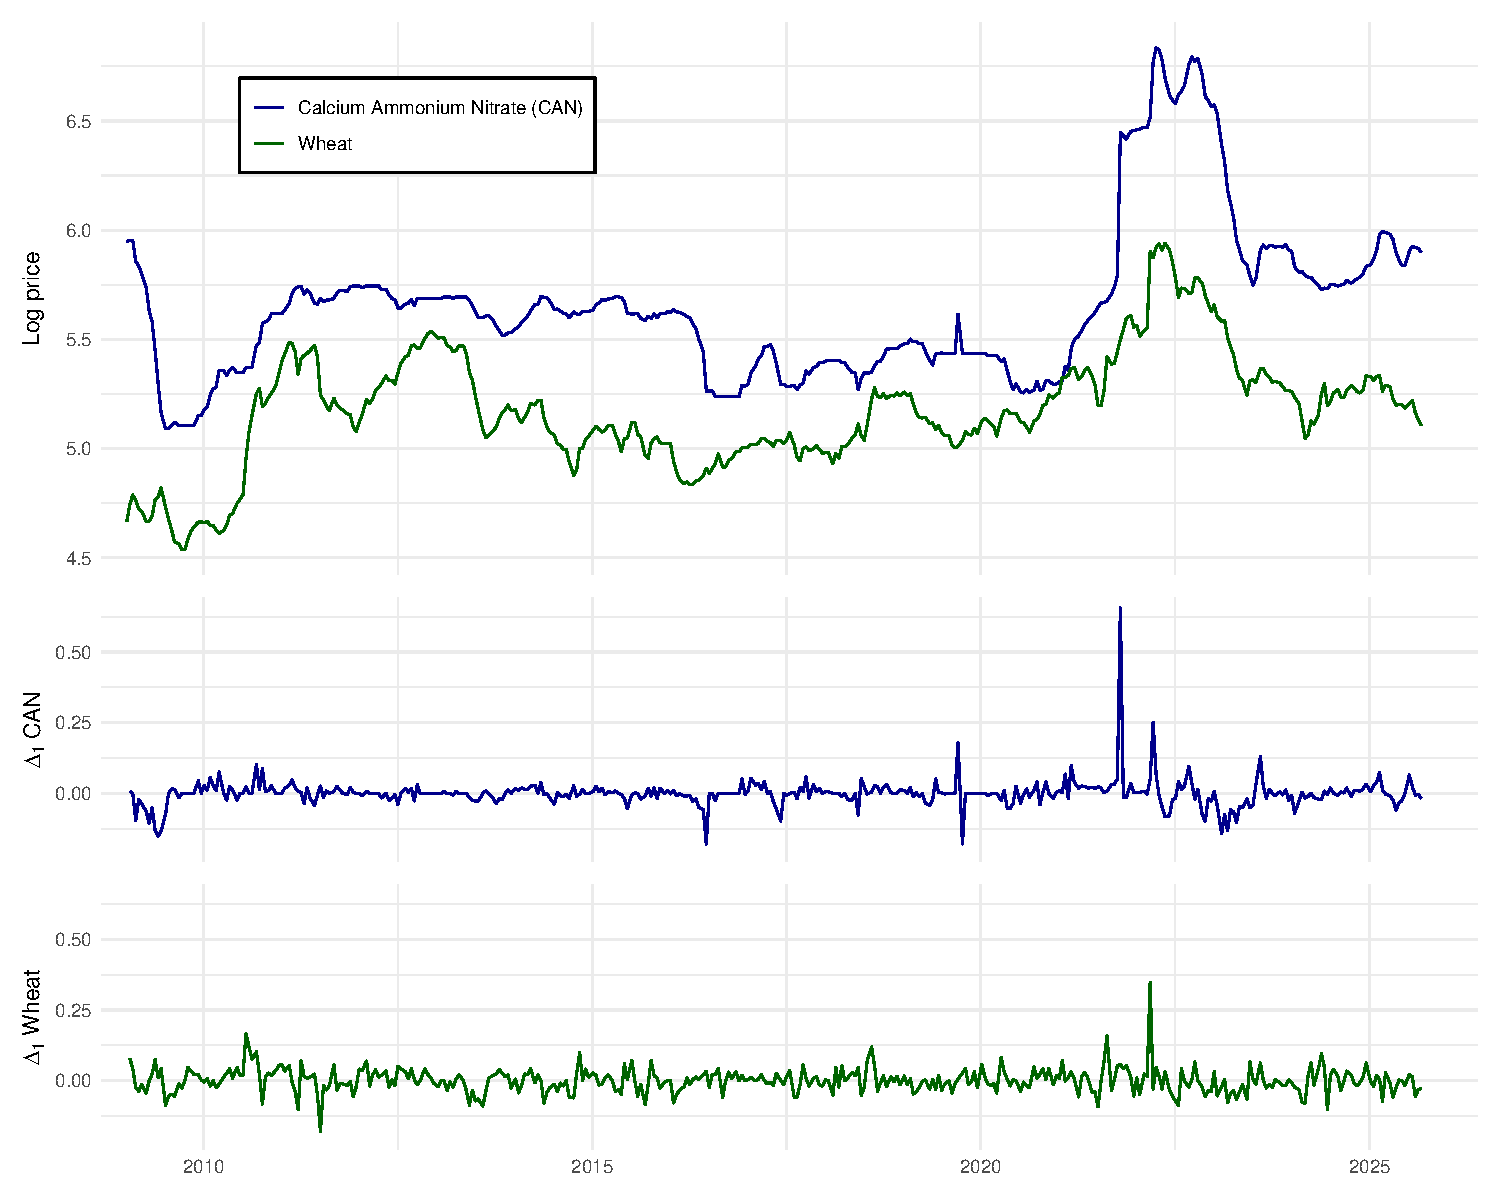
\includegraphics[width=0.85\textwidth]{Fig_CombinedPrices.pdf}
    \caption{CAN and wheat prices (Jan 2009 -- Nov 2025)}
\end{figure}
\end{frame}

% ============================================================
% 6. RESULTS
% ============================================================
\section{Results}

\begin{frame}{Production Function}
\begin{columns}[T]
\column{0.55\textwidth}
\small
\begin{table}
\centering
\begin{tabular}{lcc}
\toprule
 & Prod.\ fn. & Var.\ fn. \\
\midrule
Intercept & $-0.464^{**}$ & 0.087 \\
$N^{0.5}$ & $0.284^{***}$ & $0.081^{***}$ \\
$N$ & $0.026^{***}$ & $-0.003^{**}$ \\
\midrule
Adj.\ R$^2$ & 0.863 & 0.093 \\
N obs. & 1,609 & 1,609 \\
\bottomrule
\end{tabular}
\end{table}

\column{0.43\textwidth}
\begin{itemize}
    \item N increases both mean yield and yield variability
    \item No diminishing marginal productivity within observed range
    \item Production risk increases with N application
\end{itemize}
\end{columns}
\end{frame}

\begin{frame}{Contract Pricing}
\begin{columns}[T]
\column{0.4\textwidth}
\begin{table}
\centering
\small
\begin{tabular}{ccc}
\toprule
Quantile & Strike & Premium \\
 & (\euro/kg) & (\euro/kg) \\
\midrule
0.5 & 0.355 & 0.011 \\
0.6 & 0.361 & 0.009 \\
0.7 & 0.366 & 0.007 \\
0.8 & 0.375 & 0.004 \\
0.9 & 0.389 & 0.002 \\
\bottomrule
\end{tabular}
\end{table}

\column{0.58\textwidth}
\begin{itemize}
    \item Strike prices based on simulated CAN price quantiles
    \item Higher strike $\rightarrow$ lower premium (less likely to trigger)
    \item Premiums are small relative to fertilizer costs
\end{itemize}
\end{columns}
\end{frame}

\begin{frame}{Results: EUT -- Broad Framing}
\small
\begin{table}
\centering
\resizebox{\textwidth}{!}{%
\begin{tabular}{lccccccc}
\toprule
 & No contract & Forward & \multicolumn{5}{c}{Adjusted contract (strike price)} \\
\cmidrule(lr){4-8}
$r$ & & contract & 0.355 & 0.361 & 0.368 & 0.376 & 0.388 \\
\midrule
0.00001 & 1162.43 & 1160.01 & 1162.31 & 1162.57 & \textbf{1162.95} & 1162.21 & 1162.41 \\
0.0001 & 1158.02 & 1155.38 & 1157.77 & 1158.05 & \textbf{1158.45} & 1157.73 & 1157.95 \\
0.001 & 1113.95 & 1109.05 & 1112.32 & 1112.81 & \textbf{1113.42} & 1112.90 & 1113.37 \\
\bottomrule
\end{tabular}%
}
\end{table}

\vspace{0.5em}
\begin{itemize}
    \item Adjusted contract yields \textbf{highest CE} across risk aversion levels
    \item Forward contract yields \textbf{lowest CE} -- eliminates natural price hedge
    \item But differences are \textbf{small} ($<$4 \euro/ha)
\end{itemize}
\end{frame}

\begin{frame}{Results: CPT -- Broad Framing}
\begin{table}
\centering
\small
\begin{tabular}{cccccccc}
\toprule
 & No contract & Forward & \multicolumn{5}{c}{Adjusted contract} \\
\cmidrule(lr){4-8}
 & & contract & 0.355 & 0.361 & 0.368 & 0.376 & 0.388 \\
\midrule
$V$ & $-2.43$ & $-2.48$ & $-2.44$ & $-2.42$ & $-2.44$ & $-2.46$ & $-2.45$ \\
\bottomrule
\end{tabular}
\end{table}

\vspace{0.5em}
\begin{itemize}
    \item \textbf{All prospect values are negative} -- perceived as losses relative to reference point
    \item Adjusted contract is \textbf{not attractive} under CPT preferences
    \item Consistent across alternative parametrizations ($\alpha$, $\lambda$, $\gamma$)
    \item Exception: loss-seeking behavior ($\lambda < 1$) -- atypical case
\end{itemize}
\end{frame}

\begin{frame}{Results: Narrow Framing}
\begin{columns}[T]
\column{0.48\textwidth}
\textbf{EUT:}
\begin{itemize}
    \item Forward contract yields \textbf{highest CE}
    \item Opposite to broad framing!
    \item Without natural hedge, fixing price is optimal
    \item Adjusted contract offers no benefit
\end{itemize}

\column{0.48\textwidth}
\textbf{CPT:}
\begin{itemize}
    \item All prospect values \textbf{negative}
    \item Adjusted contract unattractive
    \item Consistent with low observed adoption rates
\end{itemize}
\end{columns}

\vspace{1em}
\begin{alertblock}{Key insight}
Under narrow framing, neither EUT nor CPT support the adjusted contract $\rightarrow$ may explain why farmers do not adopt input price risk management tools.
\end{alertblock}
\end{frame}

\begin{frame}{Summary of Results}
\begin{table}
\centering
\begin{tabular}{lcc}
\toprule
 & Broad framing & Narrow framing \\
\midrule
\textbf{EUT} & Adjusted contract & Forward contract \\
 & (marginal benefit) & preferred \\
\midrule
\textbf{CPT} & Not attractive & Not attractive \\
 & (all $V < 0$) & (all $V < 0$) \\
\bottomrule
\end{tabular}
\end{table}

\vspace{0.5em}
\begin{itemize}
    \item Input price risk has a \textbf{limited impact} on overall farm profit variability
    \item Profit variability mainly driven by \textbf{output prices and yields}
    \item A more \textbf{holistic approach} covering both input and output risk may be needed
\end{itemize}
\end{frame}

% ============================================================
% 7. DISCUSSION & NEXT STEPS
% ============================================================
\section{Discussion \& Next Steps}

\begin{frame}{Discussion}
\textbf{Key takeaways:}
\begin{itemize}
    \item Framing matters: broad vs.\ narrow framing leads to \textbf{opposite conclusions} under EUT
    \item CPT consistently predicts \textbf{low adoption} -- aligning with empirical observations
    \item Forward contracts eliminate the \textbf{natural price hedge} (fertilizer--wheat correlation)
    \item Input price risk alone may be \textbf{insufficient} to justify contract adoption
\end{itemize}

\vspace{0.5em}
\textbf{Limitations:}
\begin{itemize}
    \item Single crop, single input simplification
    \item EPIC model may underestimate yields and yield variability
    \item Simulated price distribution shows upward shift vs.\ observed
    \item CPT results sensitive to reference point specification
\end{itemize}
\end{frame}

\begin{frame}{Next Steps}
\begin{itemize}
    \item Extend to \textbf{joint input--output price risk management}
    \item Consider \textbf{multi-crop} and \textbf{multi-input} settings
    \item Explore \textbf{endogenous reference points} (K\H{o}szegi--Rabin)
    \item Validate with \textbf{farmer survey data} on preferences and framing
    \item Consider \textbf{dynamic} contracting decisions (multi-period)
\end{itemize}
\end{frame}

% ============================================================
% THANK YOU
% ============================================================
\begin{frame}{}
\centering
\vspace{2cm}
{\Large \textbf{Thank you!}}

\vspace{1.5cm}
Riccardo Spada \\
\texttt{riccardo.spada@wur.nl} \\
\vspace{0.5em}
Business Economics Group \\
Wageningen University \& Research

\vspace{1em}
\small AgEnRes Project (No.\ 101136474)
\end{frame}

\end{document}
